% =====================================================================
\chapter{Implementation}
\label{ch:implementation}

\section{Backend Application Server}
\label{sec:impl-server}
The application server is written in TypeScript and runs on Node.js with
the Express framework. TypeScript was chosen over plain JavaScript
because the domain model is intricate---trips, sources, tracking states,
and their transitions---and static typing catches an entire class of
mistakes at compile time that would otherwise surface as runtime faults
on a live fleet.

Persistence goes through the Prisma ORM to PostgreSQL. Prisma generates
typed client code from the declarative schema, so a query that survives
compilation is structurally valid against the database. The 31 models of
the schema (Section~\ref{sec:design-database}) map one-to-one to Prisma
model declarations, and schema migrations are versioned alongside the
application code.

The server exposes two interfaces: a REST API (authentication, schedules,
routes, favourites, administration) and the Socket.IO realtime gateway.
Internally, the position-processing chain is implemented as a sequence of
services---ingestion, arbitration, filtering, ETA, publication---each of
which appends to the audit logs as it acts (FR-13).

\section{Traccar Integration}
\label{sec:impl-traccar}
A self-hosted Traccar instance decodes the Concox GT06S binary protocol.
The application server consumes it through the two paths designed in
Section~\ref{sec:design-acquisition}:

\begin{itemize}
  \item The \textbf{WebSocket push} path authenticates to Traccar with a
  session cookie and subscribes to its live position stream; a decoded
  fix reaches the application server within about one second.
  \item The \textbf{REST poll} path runs on a timer and reconciles the
  latest positions for all devices, guaranteeing progress when the
  socket is down. Its cadence is trip-aware: 8\,s for buses in an active
  trip or pre-trip window, 60\,s otherwise (the optimization of
  Section~\ref{sec:eval-efficiency}).
\end{itemize}

Every inbound fix---pushed, polled, or posted by a driver device---is
recorded with both its device-reported timestamp and its server-receipt
timestamp and tagged with its source. The difference between those two
timestamps is precisely the position-acquisition latency reported in
Chapter~\ref{ch:evaluation}, so the evaluation methodology was built into
the ingestion path from the start.

\section{Source Arbitration and Filtering}
\label{sec:impl-arbitration}
The arbitration routine of Section~\ref{sec:design-arbitration} runs on
every inbound fix. Health scoring is intentionally simple---recency and
validity dominate---because the failure mode it must detect is blunt: a
source going silent. The configurable priority rank prefers the hardware
tracker whenever it is healthy. During the pilot, mid-trip handovers
occurred and produced no passenger-visible discontinuity; the canonical
marker continued from the freshest healthy source, which is the exact
behaviour the design called for.

The filtering pipeline implements the four gates of
Section~\ref{sec:design-filter} with the thresholds listed in
Appendix~\ref{app:params} (accuracy soft/hard limits 120\,m/250\,m,
teleport guard 120\,km/h, movement floor 4\,m). Accepted fixes update the
canonical state, append to the per-trip location log, and refresh the
rolling speed window; rejected fixes are logged with their rejection
reason, which proved invaluable when tuning the thresholds early in the
pilot.

\section{ETA Computation}
\label{sec:impl-eta}
The estimator implements Algorithm~\ref{alg:eta} directly. Route geometry
is preprocessed once into a cumulative-distance array; per fix, the
projection and the per-stop loop are a few hundred floating-point
operations, so the estimator adds no measurable load even at full
reporting rate. Every prediction is logged with its trip, stop, predicted
instant, and confidence label, building the dataset against which
mean-absolute-error can be measured as arrivals accumulate---and from
which a learned predictor can later be trained
(Section~\ref{sec:concl-future}).

\section{Trip Lifecycle and Background Jobs}
\label{sec:impl-lifecycle}
Three scheduled jobs drive the lifecycle of
Section~\ref{sec:design-lifecycle}:

\begin{itemize}
  \item The \textbf{pre-trip job} opens the \textsc{pre\_trip} window
  ahead of each scheduled departure, computes the vehicle's
  pre-departure state (parked, approaching origin, arrived at origin),
  and promotes the trip to \textsc{running} when the bus dwells inside
  the origin geofence.
  \item The \textbf{staleness job} runs every 30\,s and flags trips whose
  latest fix has aged beyond the threshold, switching the passenger view
  to its explicit stale presentation.
  \item The \textbf{polling job} implements the trip-aware Traccar
  reconciliation cadence described above.
\end{itemize}

\section{Passenger Mobile Application}
\label{sec:impl-passenger}
The passenger application is built with React Native and Expo, targeting
Android first (the platform of essentially all pilot riders). Its
central screen is a live map showing the route polyline, its stops, and
the bus marker with a callout presenting the vehicle's label, next stop,
ETA, and current speed.

Four behaviours distinguish it from a naive tracker, each an edge
condition handled by design:

\begin{itemize}
  \item \textbf{Pre-trip awareness.} During the \textsc{pre\_trip}
  window the app renders the bus at its known pre-departure position
  (typically the depot or origin), so the map is never blank while a
  rider waits for departure (FR-7).
  \item \textbf{Staleness signalling.} When the server flags a trip
  stale, the app says so explicitly instead of letting a frozen marker
  masquerade as live data (FR-8).
  \item \textbf{Offline retention.} On a transient disconnection the app
  keeps the last known state visible, marked as such, and resumes
  seamlessly on reconnect.
  \item \textbf{Drop-off alerts.} A rider selects their stop; when the
  bus enters the 80\,m arrival radius, a push notification fires even if
  the app is backgrounded (FR-9), using a foreground location service
  for continued tracking.
\end{itemize}

The interface is fully bilingual. Every string in the application exists
in English and Bangla, switchable in-app at any time (FR-10), and place
names render in both scripts. Localization was implemented as a
first-class concern from the first screen onward---retrofitting
translation onto a finished English app tends to leave exactly the gaps
that erode user trust. Representative screens are shown in
Figure~\ref{fig:screens} (Appendix~\ref{app:screens} reproduces them at
full page width).

\begin{figure}[H]
\centering
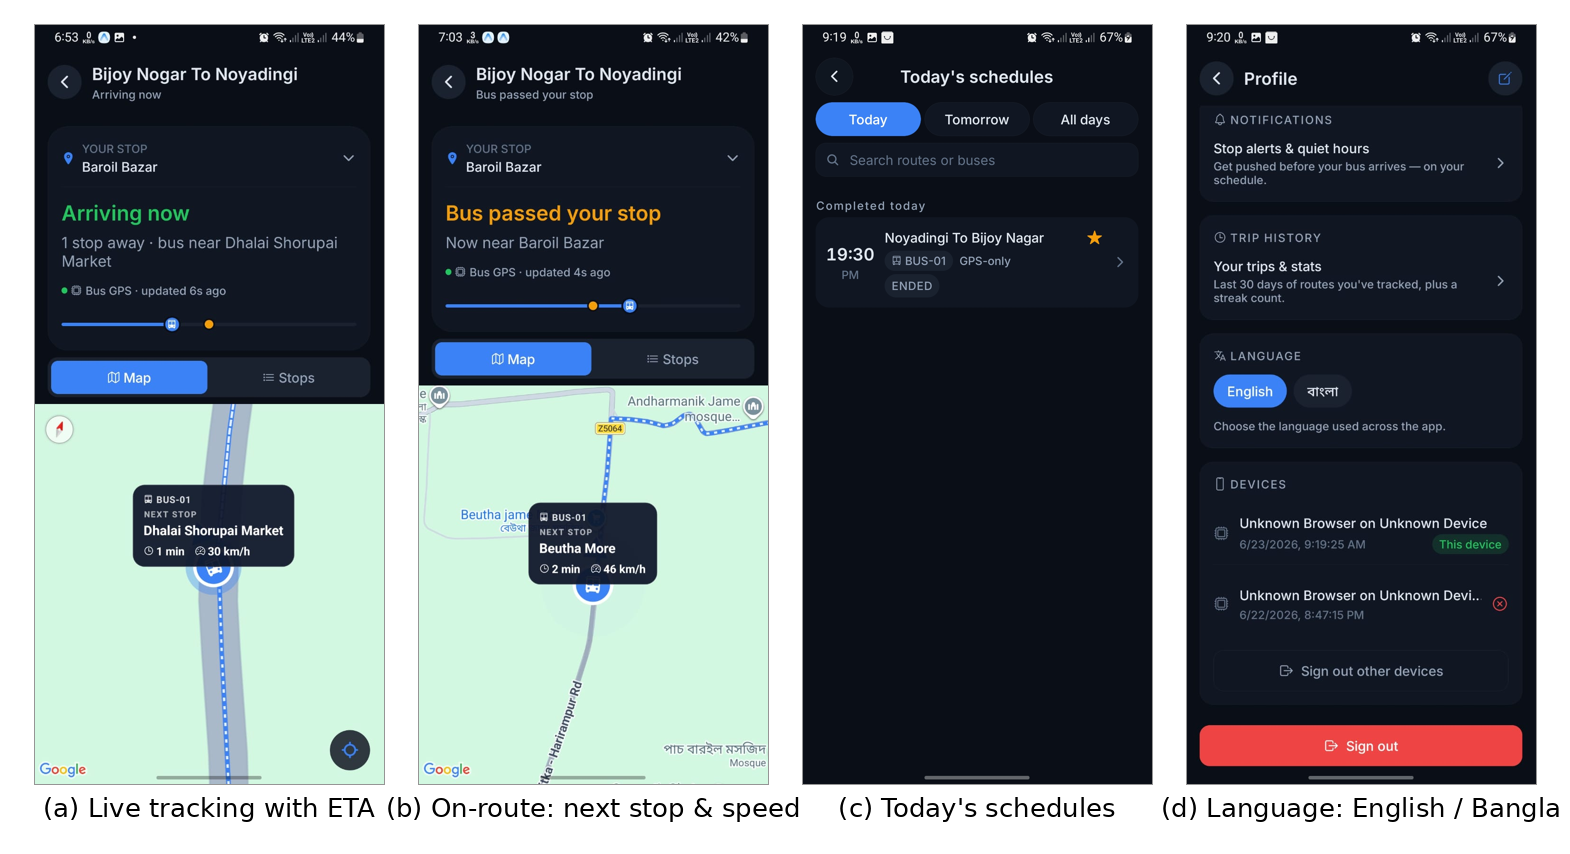
\includegraphics[width=\textwidth]{screens.png}
\caption[Screens of the bilingual passenger application]{The bilingual
passenger application. (a) live tracking of a moving bus with the
next-stop ETA; (b) on-route status showing the next stop and current
speed; (c) today's schedules; (d) the in-app English/Bangla language
toggle. Place names render in both scripts.}
\label{fig:screens}
\end{figure}

\section{Driver Mobile Application (Fallback Publisher)}
\label{sec:impl-driver}
The optional smartphone fallback of Section~\ref{sec:design-acquisition}
is served by a separate, purpose-built driver application (React Native
and Expo, distributed directly to drivers rather than publicly). It is
deliberately minimal---a login screen and a single home screen---because
its only job is to publish the bus position when a vehicle has no
working tracker. Figure~\ref{fig:driver} shows its principal states.

Four design decisions define it:

\begin{itemize}
  \item \textbf{Explicit sharing lifecycle.} The app shares nothing
  until the driver taps \emph{Start trip}, and stops the moment the
  trip ends; between trips it shows an explicit ``not sharing'' state.
  Location is therefore published only during an active trip.
  \item \textbf{Background publishing.} Unlike the passenger app, the
  driver app declares Android background-location permissions and runs
  a foreground service, with the publishing task registered at the
  global JavaScript scope so the operating system can invoke it even
  when the screen is off. Each fix is posted to the authenticated
  driver-location REST endpoint (FR-2), reading the active trip and
  credentials from secure storage.
  \item \textbf{Source selection in view.} The home screen carries the
  \emph{bus device / my phone} source selector and, while live, shows
  the driver the same telemetry the server sees---current speed, GPS
  accuracy, and seconds since the last update---so a driver can confirm
  at a glance that publishing is working.
  \item \textbf{Role guarding.} Only accounts with the driver role can
  proceed past login; any other account is refused inside the app.
\end{itemize}

\begin{figure}[H]
\centering
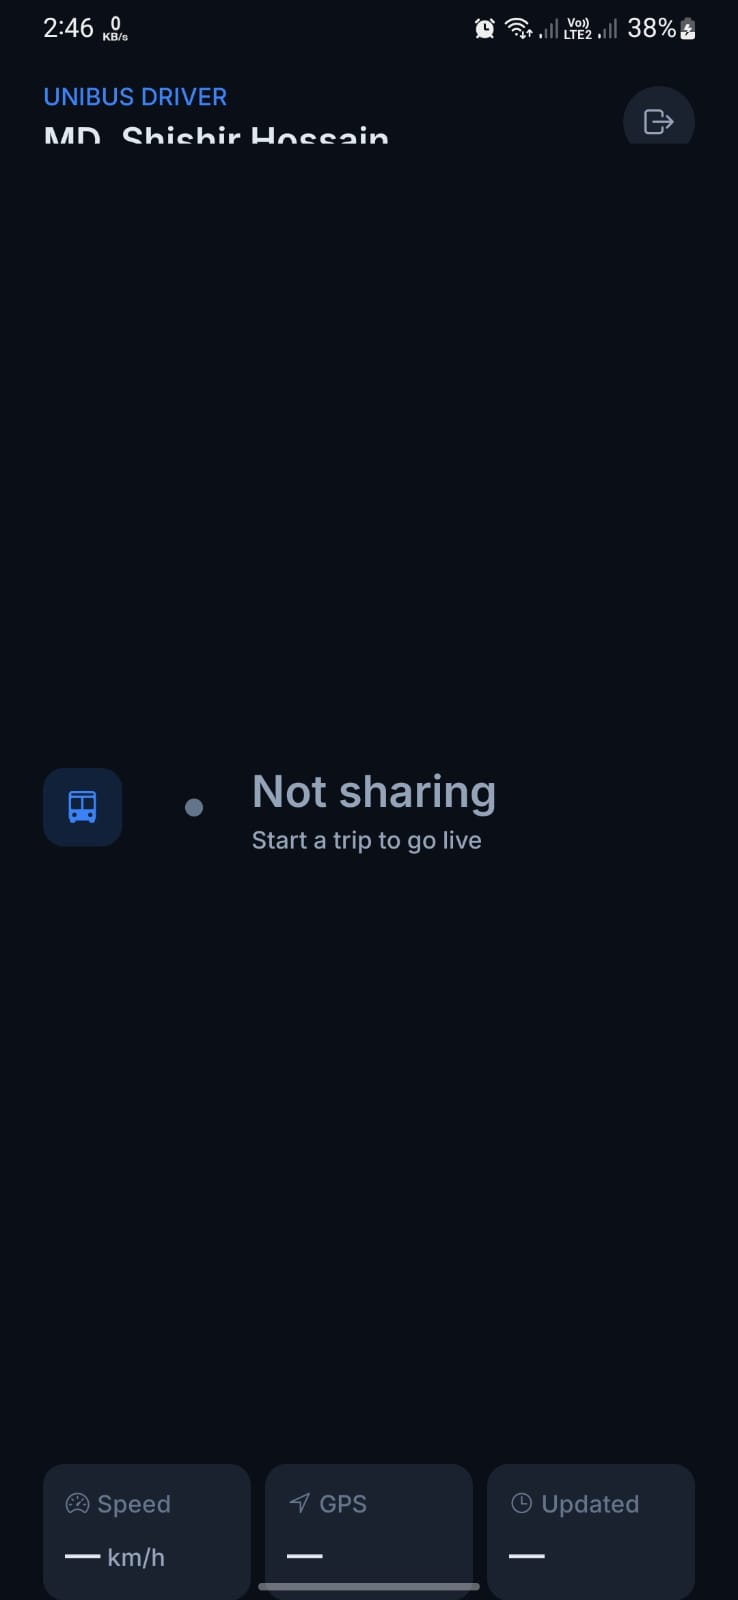
\includegraphics[width=0.235\textwidth]{driver_shots/idle.jpg}\hfill
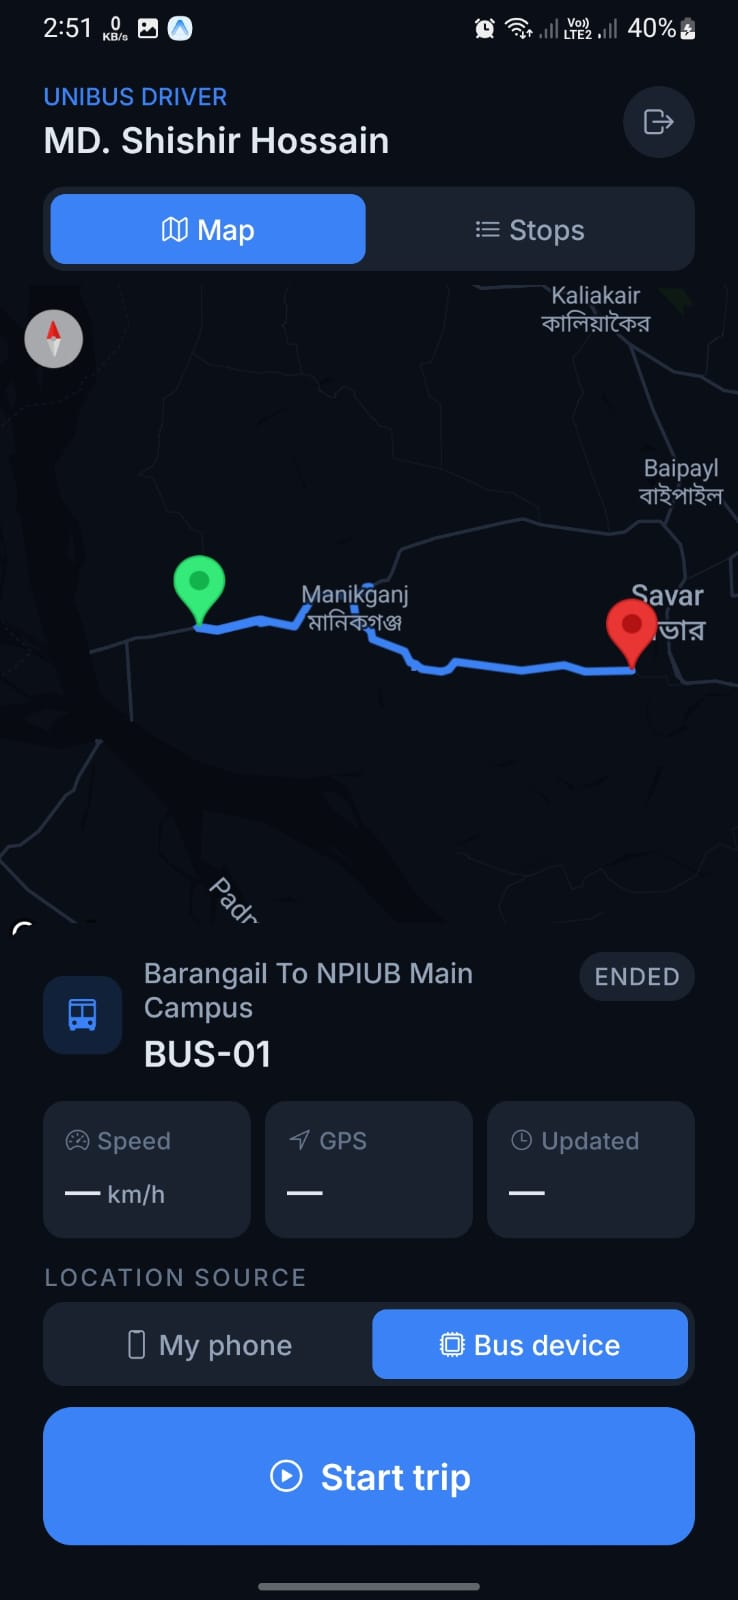
\includegraphics[width=0.235\textwidth]{driver_shots/routemap.jpg}\hfill
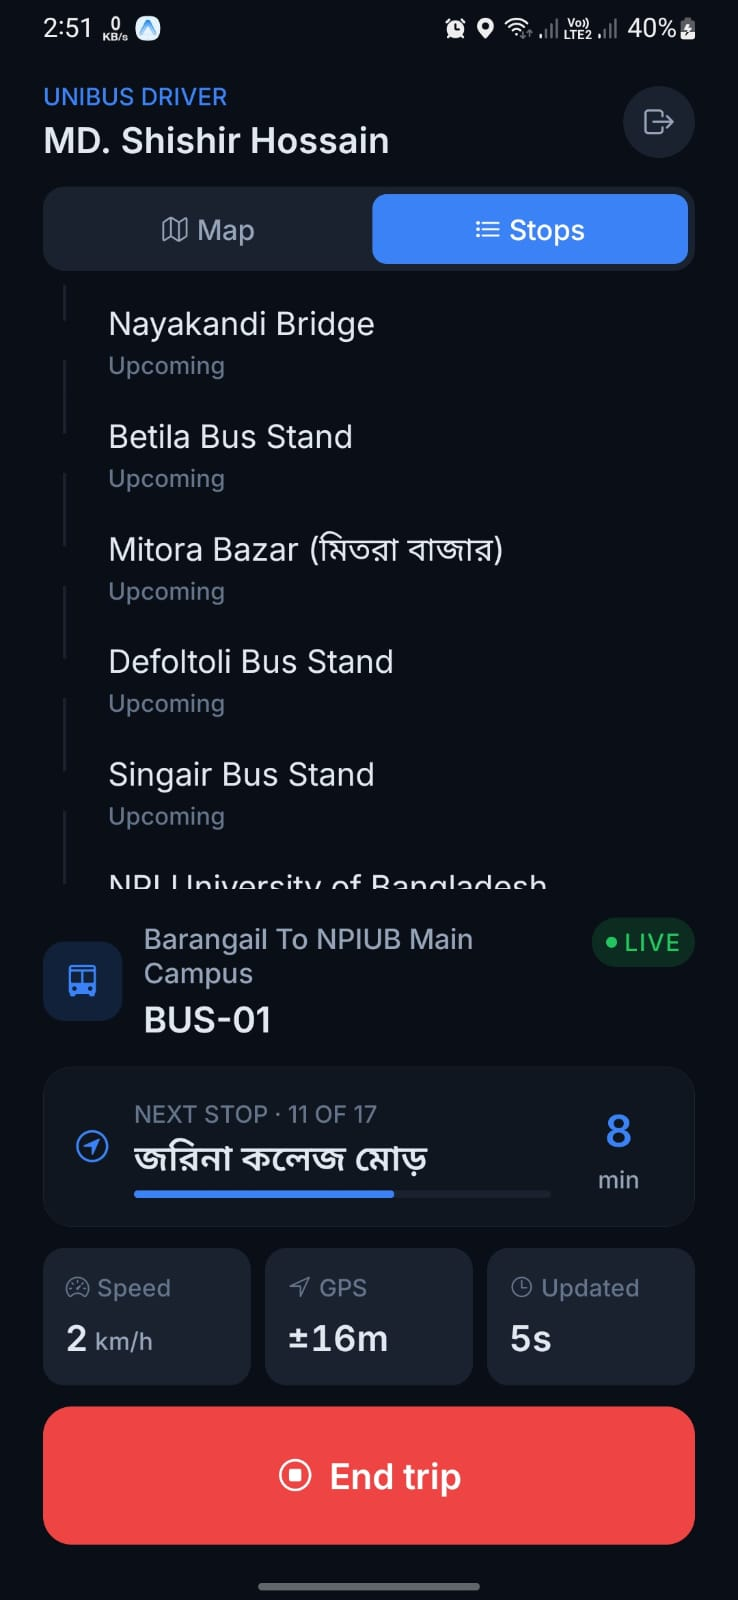
\includegraphics[width=0.235\textwidth]{driver_shots/live.jpg}\hfill

\includegraphics[width=0.235\textwidth]{driver_shots/stops.jpg}
\caption[Screens of the driver application]{The driver application.
Left to right: (a) the idle state---nothing is shared until a trip is
started; (b) the assigned trip's route map with the location-source
selector (bus device / my phone) and the \emph{Start trip} control;
(c) an active trip publishing \textsc{live}: next stop (11 of 17) with
its ETA, current speed, GPS accuracy, seconds since the last update,
and the \emph{End trip} control; (d) the stop-by-stop progress view
with done/next/upcoming states, stop names rendered in both scripts.}
\label{fig:driver}
\end{figure}

\section{Administration Console}
\label{sec:impl-admin}
The administration console is a server-rendered React application built
with Next.js. It integrates the Google Maps JavaScript API for two
map-centric tools: the \emph{live operations map}, which shows every
active vehicle in the fleet at once (FR-12), and the \emph{route
builder}, with which an administrator lays out a route's polyline and
stop sequence directly on the map. Figure~\ref{fig:admin} shows four of
its principal screens; Appendix~\ref{app:adminscreens} reproduces the
remaining management pages. Beyond the maps, the console manages
buses, GPS devices, schedules, and user roles through the same REST API
the mobile app uses (FR-11)---one API surface, two clients, no
duplicated logic.

\begin{figure}[H]
\centering
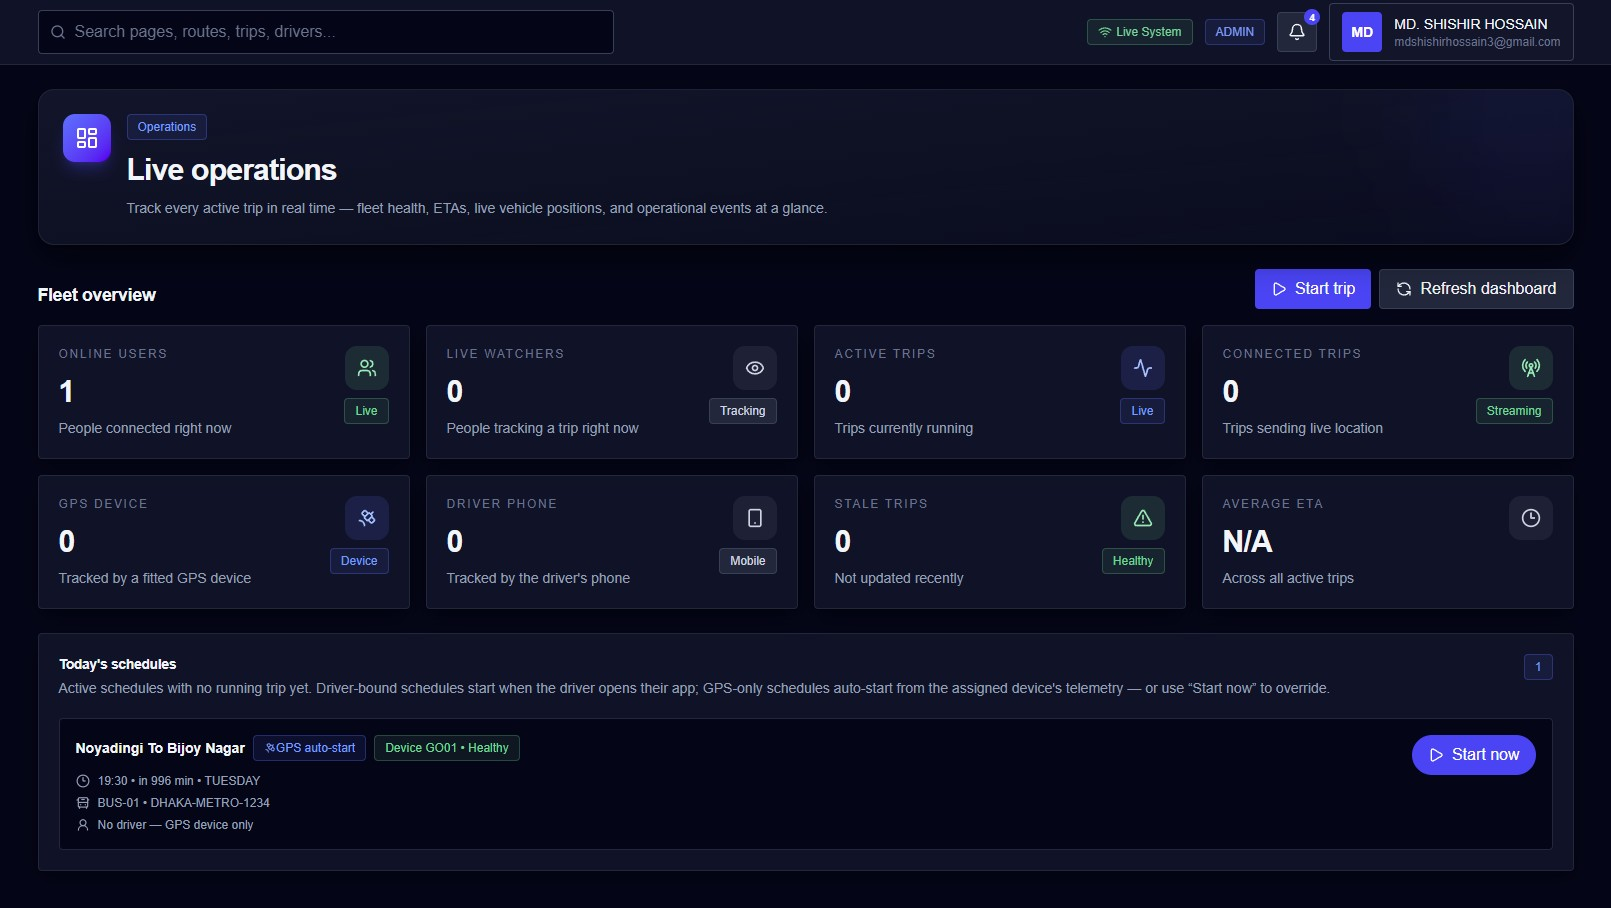
\includegraphics[width=0.49\textwidth]{admin/live_ops.jpg}\hfill
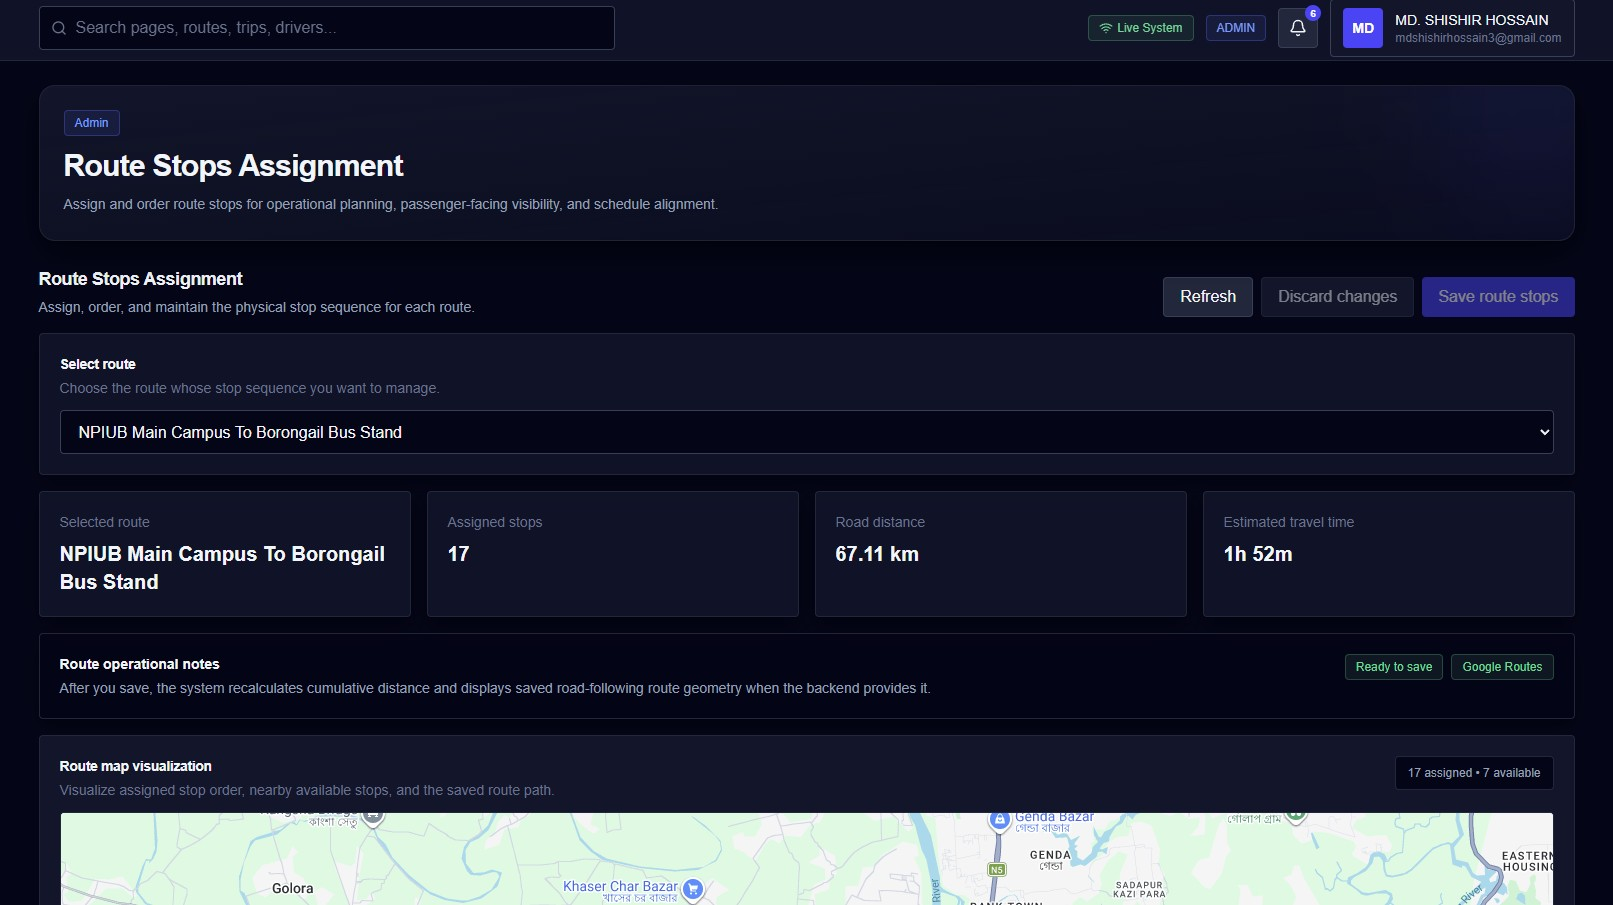
\includegraphics[width=0.49\textwidth]{admin/route_builder.jpg}\\[2mm]
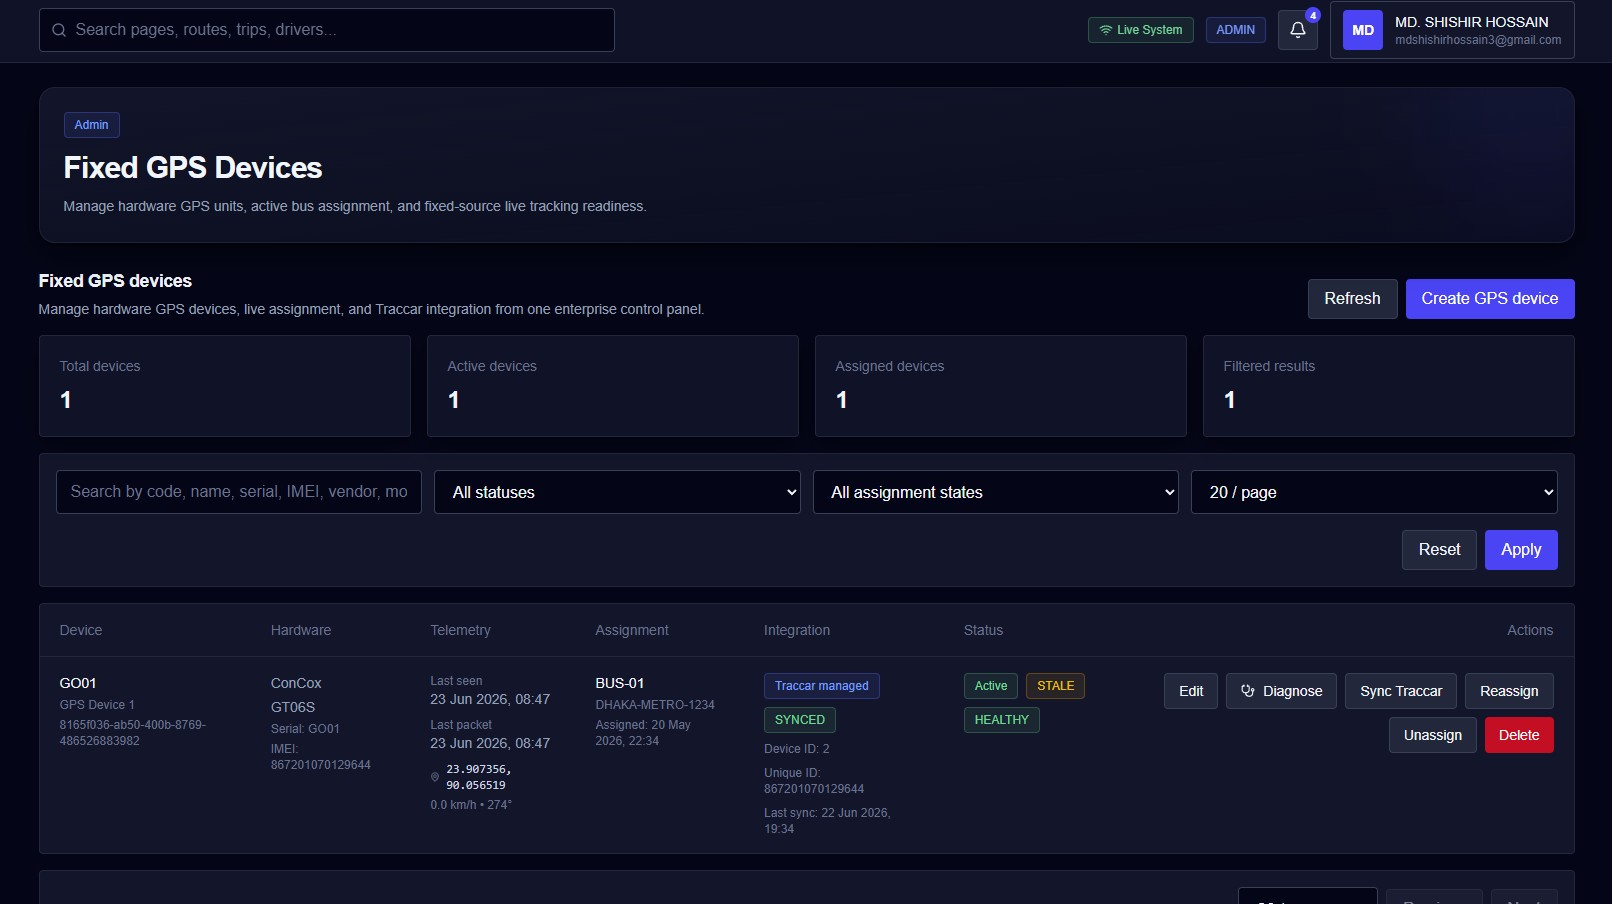
\includegraphics[width=0.49\textwidth]{admin/devices.jpg}\hfill
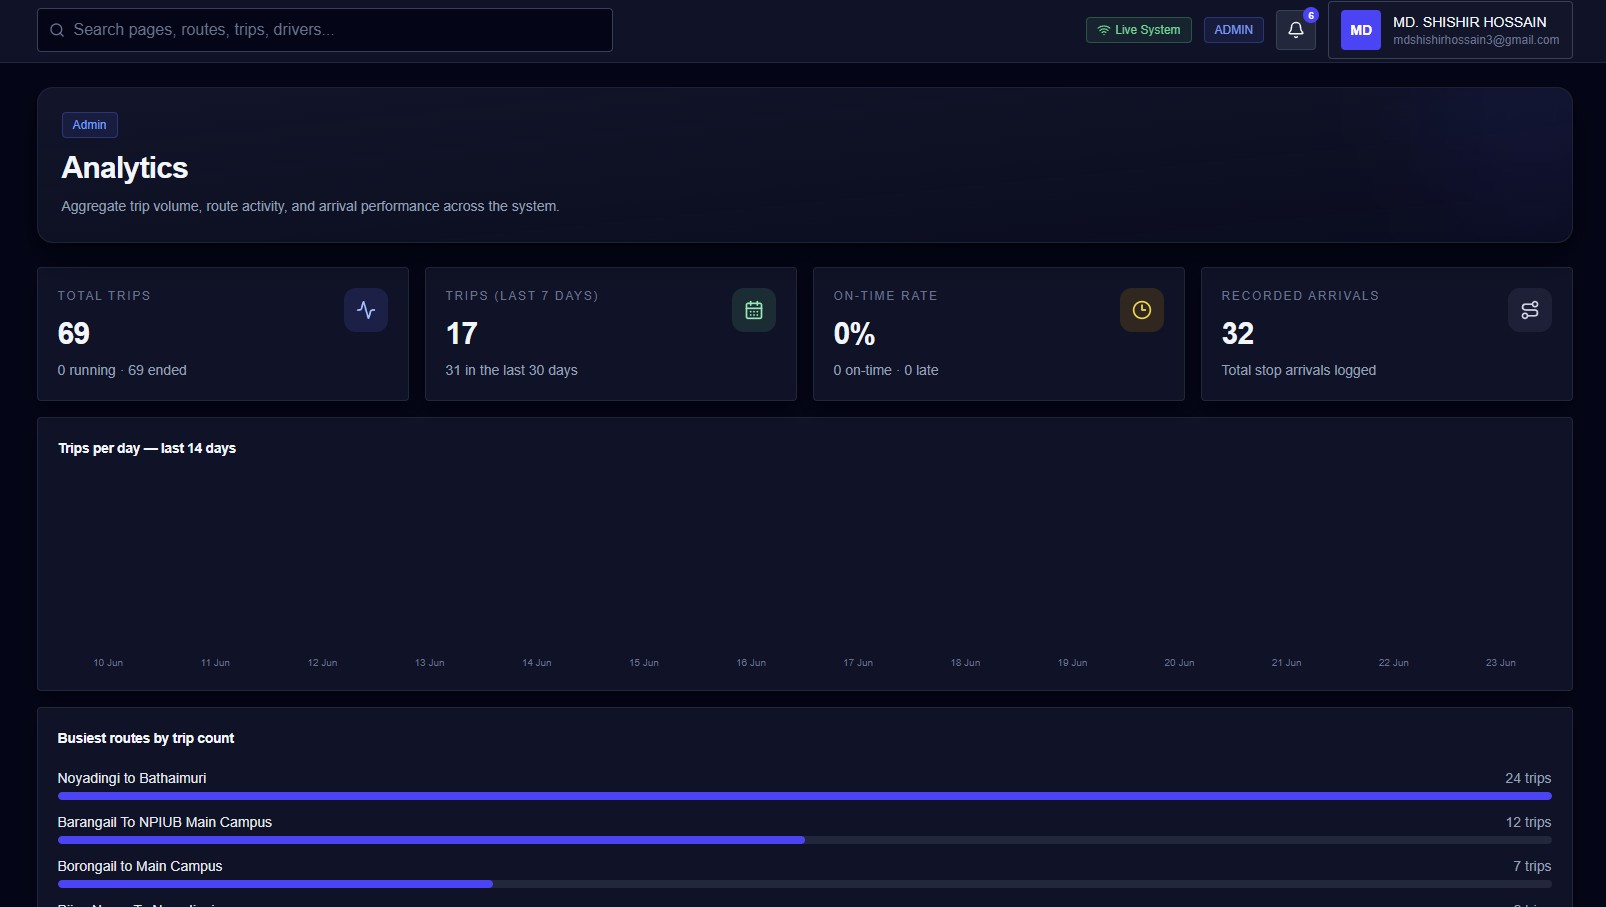
\includegraphics[width=0.49\textwidth]{admin/analytics.jpg}
\caption[Principal screens of the administration console]{Principal
screens of the administration console. Top left: the live operations
dashboard with the fleet overview and today's schedules. Top right: the
route-builder view, assigning the ordered stop sequence of a route with
its along-path distance, estimated travel time, and map visualization.
Bottom left: the fixed GPS device registry with telematics-integration
status and per-device diagnostics. Bottom right: the analytics view
aggregating trip volume, route activity, and arrival performance.}
\label{fig:admin}
\end{figure}

\section{On-Vehicle Device Configuration}
\label{sec:impl-device}
The Concox GT06S is configured over SMS, and its configuration became an
integral part of the system's efficiency story. The unit as initially
deployed transmitted a fix every 5 seconds \emph{regardless of vehicle
state}---including all night, parked in the depot. After the pilot data
quantified this waste (Section~\ref{sec:eval-efficiency}), we set an
asymmetric reporting cadence directly on the device:

\begin{itemize}
  \item \texttt{TIMER,5,300\#} --- report every 5\,s while moving, but
  only every 300\,s while static;
  \item \texttt{PARAM\#} --- read back the active configuration for
  verification;
  \item \texttt{STATUS\#} --- report battery and GSM/GPS state;
\end{itemize}

each acknowledged by return SMS (the full command set appears in
Appendix~\ref{app:sms}). We verified the change from two independent
vantage points---the per-position timestamps in Traccar's report view
and the server's own ingest log---confirming parked-state fixes spaced
by minutes rather than seconds, while a live test drive still produced
dense five-second fixes. A low-frequency heartbeat keeps the device
visible online between reports. Wiring the ignition (ACC) line for
engine-state-triggered sleep is identified as future work.

\section{Deployment}
\label{sec:impl-deploy}
The entire backend---application server, Traccar, PostgreSQL, and
Redis---runs on a single low-cost virtual private server, satisfying
NFR-3. The passenger application is distributed as an Android APK built
through the Expo Application Services build pipeline; the administration
console is served from the same VPS. No managed cloud services, message
queues, or third-party realtime providers are involved: the design goal
that a university could replicate this deployment for the cost of one
small server and one tracker per bus held from the first day of the
pilot to the last.

\section{Summary}
This chapter described the realization of the design: the TypeScript
application server and its typed persistence layer, the dual push/poll
Traccar integration with per-fix latency instrumentation, the
arbitration and filtering services, the direct implementation of the ETA
algorithm, the three lifecycle jobs, the bilingual passenger application
with its four edge-condition behaviours, the dedicated driver
application that implements the fallback publishing path, the
administration console, the SMS-based tracker configuration, and the
single-server deployment. The next chapter evaluates the deployed whole
on the real fleet.
